% TikZ architecture diagram for LST paper
% Compile standalone or \input{} into the main paper
% Requires: \usepackage{tikz}, \usetikzlibrary{shapes,arrows.meta,positioning,calc,fit}

\documentclass[border=5pt]{standalone}
\usepackage{tikz}
\usetikzlibrary{shapes,arrows.meta,positioning,calc,fit,backgrounds}
\usepackage{amsmath}

\begin{document}

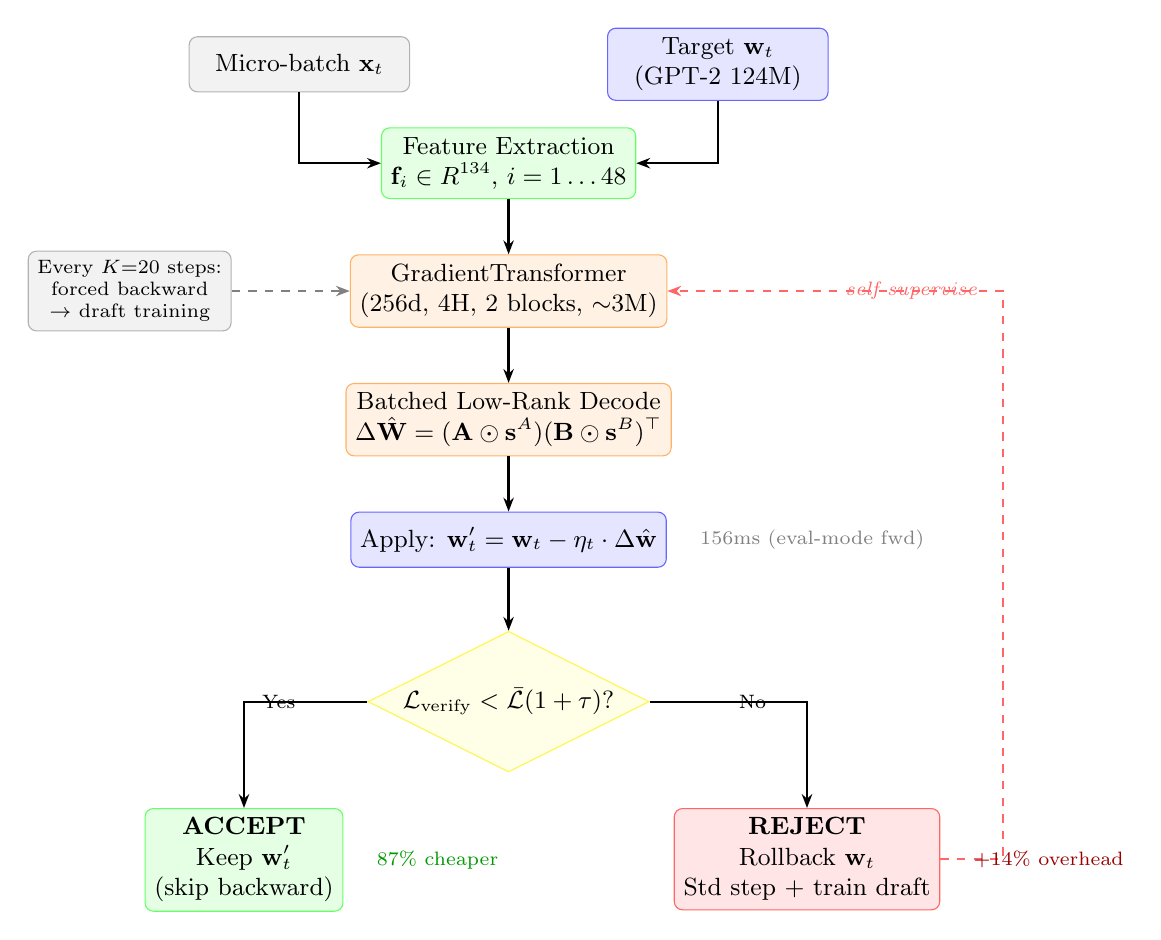
\begin{tikzpicture}[
    node distance=0.8cm and 1.2cm,
    box/.style={draw, rounded corners=3pt, minimum width=2.8cm, minimum height=0.7cm, align=center, font=\small},
    bluebox/.style={box, fill=blue!10, draw=blue!60},
    orangebox/.style={box, fill=orange!10, draw=orange!60},
    greenbox/.style={box, fill=green!10, draw=green!60},
    redbox/.style={box, fill=red!10, draw=red!60},
    graybox/.style={box, fill=gray!10, draw=gray!60},
    decision/.style={draw, diamond, aspect=2, fill=yellow!10, draw=yellow!70, minimum width=2cm, align=center, font=\small, inner sep=1pt},
    arr/.style={-{Stealth[length=5pt]}, thick},
    darr/.style={-{Stealth[length=5pt]}, thick, dashed},
]

% Layer 1: Inputs
\node[graybox] (batch) {Micro-batch $\mathbf{x}_t$};
\node[bluebox, right=2.5cm of batch] (weights) {Target $\mathbf{w}_t$\\(GPT-2 124M)};

% Layer 2: Feature Extraction
\node[greenbox, below=0.8cm of $(batch)!0.5!(weights)$] (features) {Feature Extraction\\$\mathbf{f}_i \in \mathbb{R}^{134}$, $i=1\ldots48$};

% Layer 3: Draft Model
\node[orangebox, below=0.7cm of features] (draft) {GradientTransformer\\(256d, 4H, 2 blocks, $\sim$3M)};

% Layer 4: Decode
\node[orangebox, below=0.7cm of draft] (decode) {Batched Low-Rank Decode\\$\Delta\hat{\mathbf{W}} = (\mathbf{A} \odot \mathbf{s}^A)(\mathbf{B} \odot \mathbf{s}^B)^\top$};

% Layer 5: Apply
\node[bluebox, below=0.7cm of decode] (apply) {Apply: $\mathbf{w}_t' = \mathbf{w}_t - \eta_t \cdot \Delta\hat{\mathbf{w}}$};

% Layer 6: Verify
\node[decision, below=0.8cm of apply] (verify) {$\mathcal{L}_{\mathrm{verify}} < \bar{\mathcal{L}}(1 + \tau)$?};

% Layer 7: Accept / Reject
\node[greenbox, below left=0.9cm and 1.2cm of verify, minimum width=2.2cm] (accept) {\textbf{ACCEPT}\\Keep $\mathbf{w}_t'$\\(skip backward)};
\node[redbox, below right=0.9cm and 1.2cm of verify, minimum width=2.2cm] (reject) {\textbf{REJECT}\\Rollback $\mathbf{w}_t$\\Std step + train draft};

% Arrows
\draw[arr] (batch) |- (features);
\draw[arr] (weights) |- (features);
\draw[arr] (features) -- (draft);
\draw[arr] (draft) -- (decode);
\draw[arr] (decode) -- (apply);
\draw[arr] (apply) -- (verify);
\draw[arr] (verify) -| node[near start, left, font=\scriptsize] {Yes} (accept);
\draw[arr] (verify) -| node[near start, right, font=\scriptsize] {No} (reject);

% Feedback arrow from reject to draft
\draw[darr, red!60] (reject.east) -- ++(0.8,0) |- node[near end, right, font=\scriptsize\itshape] {self-supervise} (draft.east);

% Timing annotations
\node[right=0.3cm of apply, font=\scriptsize\color{gray}] {156ms (eval-mode fwd)};
\node[right=0.3cm of accept, font=\scriptsize\color{green!60!black}] {87\% cheaper};
\node[right=0.3cm of reject, font=\scriptsize\color{red!60!black}] {+14\% overhead};

% K-step supervision annotation
\node[graybox, left=1.5cm of draft, minimum width=2cm, font=\scriptsize] (ksup) {Every $K{=}20$ steps:\\forced backward\\$\rightarrow$ draft training};
\draw[darr, gray] (ksup) -- (draft);

\end{tikzpicture}

\end{document}
